% --------------------------------------------------------------------------------

\begin{exercise}

Ein bi-parental Heap (oder Beap) ist eine Datenstruktur, wo ein Knoten zwei Eltern hat
(außer, es handelt sich um den ersten oder letzten Knoten auf einem Level) und zwei Kinder hat (außer, es ist ein Knoten am unstersten Level).

\begin{enumerate}[label = \alph*)]
  \item Sei $n$ die Anzahl der Knoten in einem Beap. Wie groß ist die Höhe des Beaps in etwa? Wie viele Elemente befinden sich auf dem letzten Level (unter der Annahme, dass dieser voll ist)?
  \item Betrachten wir nun einen MAX-Beap, d.h. einen Beap, bei dem die Einträge jedes Knotens größergleich den Einträgen in den Kindern dieses Knotens sind. Formulieren Sie einen Pseudocode für die Prozedur MAX-BEAPIFY, wobei das Feld $A$ und der Index $i$ gegeben sind, die Teil-Beaps mit den Wurzeln LEFT[$i$] und RIGHT[$i$] MAX-Beaps sind, der Eintrage $A[i]$ aber möglicherweise kleiner als die Einträge in den Kindern sein kann.
\end{enumerate}
\end{exercise}

% --------------------------------------------------------------------------------


\begin{solution}
\phantom{}
\begin{center}
  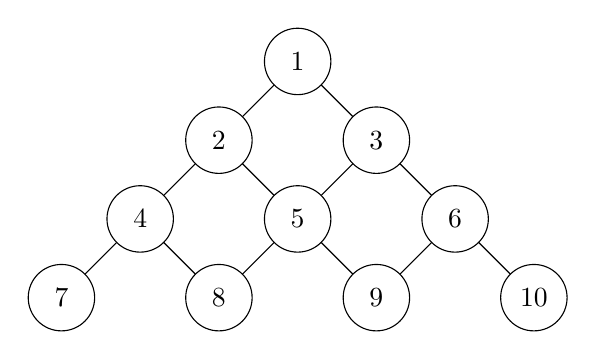
\begin{tikzpicture}

    \coordinate (x_1) at ( 0,  0);
    \coordinate (x_2) at (-1, -1);
    \coordinate (x_3) at ( 1, -1);
    \coordinate (x_4) at ( -2, -2);
    \coordinate (x_5) at ( 0, -2);
    \coordinate (x_6) at ( 2, -2);
    \coordinate (x_7) at (-3, -3);
    \coordinate (x_8) at (-1, -3);
    \coordinate (x_9) at (1, -3);
    \coordinate (x_10) at (3, -3);

    \draw (x_1) -- (x_2) -- (x_4) -- (x_7);
    \draw (x_1) -- (x_3) -- (x_6) -- (x_10);
    \draw (x_2) -- (x_5) -- (x_9);
    \draw (x_3) -- (x_5) -- (x_8);
    \draw (x_4) -- (x_8);
    \draw (x_6) -- (x_9);

    \filldraw [color = black, fill = white] (x_1) circle (12 pt) node {$1$};
    \filldraw [color = black, fill = white] (x_2) circle (12 pt) node {$2$};
    \filldraw [color = black, fill = white] (x_3) circle (12 pt) node {$3$};
    \filldraw [color = black, fill = white] (x_4) circle (12 pt) node {$4$};
    \filldraw [color = black, fill = white] (x_5) circle (12 pt) node {$5$};
    \filldraw [color = black, fill = white] (x_6) circle (12 pt) node {$6$};
    \filldraw [color = black, fill = white] (x_7) circle (12 pt) node {$7$};
    \filldraw [color = black, fill = white] (x_8) circle (12 pt) node {$8$};
    \filldraw [color = black, fill = white] (x_9) circle (12 pt) node {$9$};
    \filldraw [color = black, fill = white] (x_10) circle (12 pt) node {$10$};

\end{tikzpicture}
 \\
  Ein vollständiger Beap mit Indizierung, die Datenfeldposition des Elements angibt.
\end{center}



\begin{enumerate}[label = \alph*)]
  \item Bezeichne also $n$ die Anzahl der Knoten und $k_i$ die Anzahl der Knoten auf dem $i-$ten Level. Unter der Annahme, dass das letzte Level voll ist, was bei der gegebenen Definition immer der Fall ist, sehen wir, dass $k_i = i$. Bezeichne nun $h$ die Höhe eines Beaps, dann erhalten wir zunächst für diesen Spezialfall

  \begin{align*}
    n
    =
    \sum_{i=1}^h i
    =
    \frac{h(h+1)}{2}
  \end{align*}

  Umformen liefert nun

  \begin{align*}
    n
    &=
    \frac{h(h+1)}{2}
    \iff
    h^2 + h - 2n = 0 \\
    \stackrel{h > 0}{\iff}
    h &= -\frac{1}{2} + \sqrt{\frac{1}{4} + 2n}
    = \frac{\sqrt{1 + 8n} - 1}{2}
  \end{align*}

Falls unser Beap mit $n$ Knoten nicht Vollständig ist, können wir den Beap mit $n^+ > n$ Knoten betrachten der Vollständig ist (in dem Sinn, dass das letzte Level voll aufgefüllt wurde). Dieser hat klarerweise die selbe Höhe. Wenn wir auch noch den Vollständigen Beap mit $n^- < n$ Knoten betrachten, wobei hier genau das letze Level geleert wurde, erhalten wir für die Höhe:

\begin{align*}
 \frac{\sqrt{1 + 8n^-} - 1}{2}
 \leq
 \frac{\sqrt{1 + 8n} - 1}{2}
 \leq
 \frac{\sqrt{1 + 8n^+} - 1}{2} \\
  h(n^-) = \frac{\sqrt{1 + 8n^-} - 1}{2} + 1
  =
  h(n)
  =
  h(n^+) = \frac{\sqrt{1 + 8n^+} - 1}{2}
\end{align*}

Somit ist die Höhe des Beaps mit $n$ Knoten

\begin{align*}
  h(n)
  =
  \Big\lceil \frac{\sqrt{1 + 8n} - 1}{2}\Big\rceil
\end{align*}
  \item Wir orientieren uns an der Prozedur $\textsc{ErzeugeHalde}$ aus dem Skript. Wir nehmen also an, dass der Beap als Datenfeld realisiert ist und wir Identifizieren die Elemente mit ihrer Position in dem Datenfeld. Dabei gehen wir wie bei den Halden vor. Zunächst definieren wir uns eine Funktion sowie einige Prozeduren.

  \begin{align*}
    \mathrm{Level}(i) := \Big\lceil \frac{\sqrt{1 + 8i} - 1}{2}\Big\rceil \\
    h(i) := \frac{\sqrt{1 + 8i} - 1}{2}
  \end{align*}

  Bezeichnen wir (sofern vorhanden) den rechten Elternteil als Vater und den linken Elternteil als Mutter sowie das rechte Kind als Sohn und das linke Kind als Tochter erhalten wir die Prozeduern



    \begin{algorithmic}[1]
        \Procedure{Mutter}{$i$}
            \If{Level($i$)-1 = h($i-1$)}
            \Comment Es gibt keine Mutter, da Element ganz links im Level
                \State \Return NIL
            \Else
                \State \Return $i$- Level($i$)
            \EndIf
        \EndProcedure
    \end{algorithmic}

\phantom{}

    \begin{algorithmic}[1]
        \Procedure{Vater}{$i$}
            \If{Level($i$) = h($i$)}
            \Comment Es gibt keinen Vater, da Element ganz rechts im Level
                \State \Return NIL
            \Else
                \State \Return $i$ - Level($i$) + 1
            \EndIf
        \EndProcedure
    \end{algorithmic}

\phantom{}

    \begin{algorithmic}[1]
        \Procedure{Tochter}{$i$, A}
            \If{$i$ + Level($i$) $>$ A.HLänge}
            \Comment Es gibt keine Tochter
                \State \Return NIL
            \Else
                \State \Return $i$ + Level($i$)
            \EndIf
        \EndProcedure
    \end{algorithmic}

\phantom{}

    \begin{algorithmic}[1]
        \Procedure{Sohn}{$i$, A}
            \If{$i$ + Level($i$) + 1 $>$ A.HLänge}
            \Comment Es gibt keinen Sohn
                \State \Return NIL
            \Else
                \State \Return $i$ + Level($i$) + 1
            \EndIf
        \EndProcedure
    \end{algorithmic}


Nun können wir unsere Prozendur mittels Abwärtskorrektur realisieren

\begin{algorithm}
  \caption{Erstelle MAX-Beaps von Wurzel $A[i]$ ausgehend}
  \begin{algorithmic}[1]
      \Procedure{Max-Beapify}{$i$}
          \State A.HLänge := A.Länge
          \State Vertausche A[1] und A[i]
          \State $k :=$ \textsc{Vater}(A.HLänge)
          \If{$k$ = NIL}
            \State $k :=$ \textsc{Mutter}(A.HLänge)
          \EndIf
          \If{Level(A.HLänge) $>$ 2}
            \For{j = k ,..., 2}
              \State \textsc{Abwärtskorrigieren(A,$i$)}
            \EndFor
          \EndIf
      \EndProcedure
  \end{algorithmic}
\end{algorithm}

Die Prozedur $\textsc{Abwärtskorrigieren}$ ist dabei jene aus dem Skript, wobei man die Prozedueren $\textsc{Links}$ und $\textsc{Rechts}$ durch $\textsc{Tochter}$ sowie $\textsc{Sohn}$ ersetzen muss.

\includegraphicsboxed{ ../../../Fundament-LaTeX/images/DGA/DGA - Algorithmus 22 - Extraktion des Maximums aus Prioritätswarteschlange}
\end{enumerate}

\end{solution}
